\chapter{Approaches to Predictive Maintenance}
\label{chapter:approaches}

The goal of \gls{pdm} is to monitor and analyze condition of a subject in order to plan a maintenance action when the subject is faulty or a failure is likely to occur soon.
This can be achieved by using \gls{ml} algorithms and historical condition monitoring data to build a model that predicts the condition --- a \gls{pdm} model.
In this chapter we describe three main approaches how to build a \acrshort{pdm} model --- fault detection (Section \ref{sec:approaches_fd}), failure prediction (Section \ref{sec:approaches_failure_prediction}) and remaining useful life (Section \ref{sec:approaches_prognostics}).
We put an emphasis on the \gls{ml} techniques used in the individual approaches and the evaluation of the built models.

\begin{introduction}

\section{Motivation}

\Acrfull{pdm} is a maintenance strategy where the goal is to monitor and analyze condition of a subject in order to plan maintenance actions at times when the subject suffers from a fault or when there is an increased probability that the subject will fail in near future.
Such maintenance strategy can significantly reduce costs and possible downtime caused by failures in comparison with other strategies such as corrective or preventive where the maintenance actions are scheduled only when the machinery fails, and thus needs a correction, or are scheduled at regular intervals.

The condition monitoring is done by collecting various kinds of data that can contain information about the health state of the subject.
The analysis can be then done by building a predictive model that is, given condition monitoring data, capable of predicting whether the subject is faulty or estimating when a failure will occur.
Nowadays, such \acrshort{pdm} models can be built utilizing \acrfull{ai}, more specifically \acrfull{ml}, techniques where the models are trained on condition monitoring and health data of multiple subjects.
Depending on what type of condition monitoring data is available, various \acrshort{ml} modeling techniques can be used.

A crucial part of \acrshort{pdm} is a performance evaluation of the built model, i.e. estimation how the model will perform in real-world.
The performance evaluation has two major goals.
The first goal is that it should serve as a way how to choose the best performing model when building models with different parameters or \acrshort{ml} algorithms.
The second goal is that the performance evaluation should be intuitively interpretable --- e.g. how much in advance is the model able to predict a failure or how often the model predicts false alarms.
As there exist various evaluation metrics which can be used for every modeling approach a good overview of different evaluation metrics and their advantages and disadvantages is crucial for a success of \acrshort{pdm} project in industry.

\section{Related Work}

Predictive maintenance has drawn huge attention in both scientific and industrial research over the past two decades.
Numerous scientific articles describing novel \acrshort{ai} approaches to \acrshort{pdm} as well as many articles describing the application of \acrshort{pdm} in various domain such as predicting failures  in wind turbines, hard drives, high-speed trains or power plants has been published in past years \cite{yuan2019, peng2018novel, kauschke2016predicting, murray2005machine, prytz2014machine, liu2017svm, xiao2016probabilistic}.
There have been published multiple reviews and surveys on predictive maintenance  systems, purposes and different approaches \cite{lei2018machinery, zhang2019data, ran2019survey, lee2014prognostics, jia2018review}.
Some works specifically focus on the application of various approaches of artificial intelligence and machine learning in predictive maintenance \cite{jahnke2015machine, korvesis2017machine, tsui2015prognostics} while other works propose novel or adjusted evaluation metrics for the individual approaches \cite{saxena2010metrics, tatbul2018precision, kauschke2015challenges, weiss1998learning}.
However, to our knowledge, there is no work that would provide an overview of multiple \acrshort{ml}-based modeling approaches and would focus at the same time on comparison of the different evaluation metrics.

\section{Goals}

The goals of this thesis are to:
\begin{itemize}
    \item give an introduction to the problematics of \acrshort{pdm};
    \item provide an overview of several different \acrshort{ml}-based modeling approaches used for building \acrshort{pdm} models;
    \item describe different evaluation metrics that can be used to assess the performance of the models built by different modeling approaches; 
    \item compare and discuss the practical application of the different evaluation metrics by conducting experiments on real-world data sets.
\end{itemize}

\section{Organization of the Thesis}

This thesis is organized as follows.
In Chapter \ref{chapter:ml} we provide a minimal theoretical background of \acrshort{ml} including the classical machine learning tasks and their evaluation metrics.
In Chapter \ref{chapter:pdm} we provide an introduction to \acrshort{pdm} in context of different maintenance strategies and we describe typical condition monitoring data used for building a \acrshort{pdm} model.
In Chapter \ref{chapter:approaches} we review different approaches to \acrshort{pdm} utilizing \acrshort{ml} techniques and we describe how the built \acrshort{pdm} models can be evaluated.
Finally, in Chapter \ref{chapter:experiments} we conduct experiments where we demonstrate the modeling approaches on real-world data sets, we compare their evaluation metrics and we discuss the metrics' practical application.

\end{introduction}

\section{Fault Detection}
\label{sec:approaches_fd}

Fault detection is an approach where the goal is to detect whether a subject suffers from a fault or a malfunction \cite{jia2018review}.
It is thus a classification problem where the features are known condition monitoring data and the target variable is a binary health label --- healthy (no fault) or faulty.
When a fault is detected a maintenance action can be immediately scheduled so that a potential failure of the subject (and thus its downtime) is avoided.

From the approaches we describe in this chapter, fault detection approach is the least restrictive regarding data requirements --- it does not require any data about the actual failures of the subjects..
Moreover, fault detection model can be build even when there are no health labels available at all.
In that case, the faults can be considered as anomalies\footnote{as the fault indeed should be rare and out of distribution of the regular behaviour} and thus the fault detection can be formulated as an anomaly detection problem.

\subsection{Data Specifications}
\label{sec:approaches_fault_detection_data}

\begin{table}
	\centering
	\caption{Example data for fault detection: (a) point-based faults, (b) range-based faults.}
    \label{tab:approaches_fault_detection_data}
    \subcaption{point-based faults}
    \label{tab:approaches_fault_detection_data_point}
    \begin{tabular}{|cccc|c|}
    \hline 
        \multicolumn{4}{|p{5cm}|}{\centering features}
        & \multicolumn{1}{|p{2.1cm}|}{\centering fault}\\\hline
        1.2  &           3.1 & $\cdots$ &      4.1 &        0 \\
        2.1  &           4.2 & $\cdots$ &      8.0 &        1 \\
    	2.0  &           2.4 & $\cdots$ &      2.2 &        0 \\
    	1.9  &           1.4 & $\cdots$ &      9.2 &        1 \\
    	1.0  &           2.7 & $\cdots$ &      2.3 &        0 \\
        $\vdots$ &      $\vdots$ & $\ddots$ & $\vdots$ & $\vdots$ \\
    \end{tabular}
    \bigskip
    \subcaption{range-based faults}
    \label{tab:approaches_fault_detection_data_range}
	\begin{tabular}{|c|c|cccc|c|}
    \hline
    subject id
    & time
    & \multicolumn{4}{|p{4cm}|}{\centering features}
    & fault\\
    \hline
    subject A & 2020-01-01 &          0.1 &         0.05 & $\cdots$ &  34.1 & 0 \\
	subject A & 2020-01-02 &          0.3 &         0.12 & $\cdots$ &  34.2 & 0 \\
    subject A & 2020-01-03 &          1.1 &         3.2  & $\cdots$ &  37.5 & 1 \\
    subject A & 2020-01-04 &          1.2 &         3.1  & $\cdots$ &  37.9 & 1 \\
    subject A & 2020-01-05 &          0.2 &         0.02 & $\cdots$ &  33.1 & 1 \\
    subject A & 2020-01-07 &          2.5 &         0.21 & $\cdots$ &  35.9 & 0 \\
    subject A & 2020-01-08 &          2.2 &         0.2  & $\cdots$ &  36.1 & 0 \\
    $\vdots$ & $\vdots$ & $\vdots$ & $\vdots$ & $\ddots$ & $\vdots$ & $\vdots$ \\
	\end{tabular}
\end{table}

Fault detection approach expects condition monitoring data as the features and optionally a binary label (healthy / faulty) as the target variable.
The health labels are not required as the faults can be regarded as the most anomalous samples.
Based on several real-world data sets for fault detection \cite{phm15, westernbearing, data_set_phm_2012, data_set_hydraulic_systems, data_set_aps_scania} we identified two types of data for fault detection --- data with range-based faults and data with point-based faults.

\begin{figure}
    \includegraphics[width=\textwidth, keepaspectratio]{%
        approaches_fault_detection_range_example.pdf}
    \centering
    \caption{Example of range-based faults in a power plant}
    \label{fig:approaches_fault_detection_range_example}
\end{figure}

\paragraph{Range-based faults}
The data for fault detection can consist of time series where at each time point there is one sample that has condition monitoring data and a separate health label.
The faults are thus located in time and they can last over multiple time points --- consecutive samples with positive health labels (fault present) can be considered as one fault.
Inspired by an article by Tatbul et al. \cite{tatbul2018precision} where the object of study are range-based anomalies, i.e. anomalies lasting in time, we call such faults range-based faults.
Figure \ref{fig:approaches_fault_detection_range_example} shows an example of range-based faults from a real-world data set containing faults in power plants \cite{phm15}.
Table  \ref{tab:approaches_fault_detection_data_range} then show an example of the format of the data with range-based faults.

\paragraph{Point-based faults}
Data with point-based faults are data where each sample that contains condition monitoring data and a health label is considered as time-independent to all the other samples.
Each fault can be then considered as a single point --- we thus call such faults point-based.
Such data set is for example a Seeded Bearing Fault Test data set from Case Western University Bearing Data Center \cite{westernbearing} where various faults were seeded in bearings and their vibration data were measured on a test apparatus.
Note, that as the vibration data are collected as signals, the data set consists of time series.
However, in contrast to data with range-based fault, here each time series corresponds to one sample and thus one health label.
An example of the format of the data with point-based faults is shown in Table \ref{tab:approaches_fault_detection_data_point}.

The range-based faults are commonly more realistic --- in real-world the faults typically do last in time.
On the other hand, the data with point-based faults can be much easier to collect --- a set of healthy and faulty subjects are inspected, e.g. in a laboratory conditions or at a workshop, as for example in case of seeded bearing fault test data set mentioned above.

The range-based faults are often converted into the point-based faults before modeling as it is easier to build a fault detection model on the point-based data than on the time-series data.
In the conversion, each range-based fault is split into multiple point-based ones (accordingly to the length of the range).
It is important to note, though, that the range-based and point-based faults should be evaluated differently as the classical metrics for classification are not suitable for evaluation of range-based faults --- they would highly favor faults with long ranges (more in Section \ref{sec:approaches_fault_detection_evaluation}).

The faults are typically rare as the subjects are most of the time  healthy\footnote{hopefully}.
Therefore, real-world data sets for fault detection are commonly highly imbalanced with the samples having a positive label (faulty) being the minority.
An exception can be data collected in laboratory conditions where for example the number of healthy and faulty samples can be the same.
Such example is a condition monitoring of hydraulic systems data set\cite{data_set_hydraulic_systems} where multiple operation modes including a healthy mode and multiple faulty modes were simulated on a testing rig of a hydraulic system where the same amount of data was collected for every operation mode.
% It is be questionable whether a data set with a lack of natural imbalance between the faulty and healthy states is suitable for building a fault detection model.

Another important aspect of data for fault detection is the availability of health labels.
As mentioned in previous chapter (Section \ref{sec:pdm_data}) the labels are typically obtained manually during e.g. corrective maintenances or by expensive methods such as disassembling of a machinery or an X-ray imaging.
Therefore, it might happen that there are either no health labels available or they are not in a sufficient quantity or even quality.

\subsection{Modeling}

Fault detection is a binary classification problem --- the goal is to build a model that predicts a binary class where the negative class corresponds to a healthy state and the positive class to a faulty state.
The choice of the specific \gls{ml} algorithm is affected by four aspects: format of the condition monitoring data (e.g. time series, spectra or simple features), type of faults (point-based faults vs range-based faults), the class imbalance and the (un)availability of the health labels.

As shown in Figure \ref{fig:pdm_model_concept} an observation\footnote{one sample in the data set that containing condition monitoring data and for which we predict the label} of a subject can consist of a simple feature vector, one dimensional structures such as a time series or frequency spectra, images such as spectrograms or even an arbitrary combination of the mentioned.
In case of a simple feature vector, classical ML algorithms such as SVM or decision trees are commonly used \cite{santos2015svm, mahadevan2009fault, zhao2012decision}.
On the other hand, deep learning algorithms such as recurrent or convolutional neural networks are used as the state-of-the-art methods for fault detection with condition monitoring data containing time series or images \cite{guo2017deep, jia2016deep, janssens2016convolutional,yuan2019}.

% TODO point-based vs range-based

As the data sets for fault detection are commonly highly imbalanced (as described in \ref{sec:approaches_fault_detection_data}) techniques to increase the capability of the supervised classification algorithms to classify the minority class are commonly used.
Such techniques include data set balancing before the training phase or a modification of the algorithm itself \cite{borovicka2012selecting}.

In case there are only few labels available or there are no labels available at all, semi-supervised and unsupervised techniques such as anomaly detection with autoencoders can be used \cite{chandola2009anomaly, yuan2019}.

\subsection{Evaluation}
\label{sec:approaches_fault_detection_evaluation}

In this section we describe how to evaluate a performance of a fault detection model.
The questions that the evaluation of a fault detection model should answer are:
\begin{itemize}
    \item What is the probability that the model will detect a fault?
    \item What is the probability that the model will predict a false alarm?
\end{itemize}

The questions above are in \gls{ml} commonly answered by precision and recall metrics.
The evaluation of point-based faults follows classical definition of precision and recall as described in Section \ref{sec:ml_evaluation} as it is a standard binary classification.
Regarding the range-based faults, we can convert them into point-based faults, and thus we can use the same classical evaluation metrics.
However, the classical evaluation metrics might lead to misleading results for range-based faults.

\begin{figure}
    \includegraphics[width=\textwidth, keepaspectratio]{%
        approaches_fault_detection_evaluation_motivation.png}
    \caption{Point-based vs range-based faults (anomalies) \cite{tatbul2018precision}.}
    \label{fig:approaches_fault_detection_evaluation_motivation}
    \centering
\end{figure}

In case of range-based faults the predictions are located in time, i.e. they have a start time and end time.
However, the predictions are made point-wise, i.e. each time point is assigned either positive or negative label.
Therefore, it might happen that a range-fault is only partially predicted (i.e. there are both positive and negative predictions during the fault).
Figure \ref{fig:approaches_fault_detection_evaluation_motivation} illustrates such problem where the range-based faults (in the figure named anomaly ranges) are only partially predicted.
The notation used in the above mentioned figure and in the rest of this section will be as follows:
\begin{itemize}
    \item $R$ and $R_i$ --- the set of real fault ranges and the $i^\text{th}$ real fault range, respectively;
    \item $P$ and $P_j$ --- the set of predicted fault range and the $j^\text{th}$ predicted fault range, respectively.
\end{itemize}
Below we define range-based recall and range-based precision metrics, for time series, respectively, as introduced by Tatbul et al. \cite{tatbul2018precision}.
If not mentioned otherwise, all the definitions and statements below are taken and paraphrased from \cite{tatbul2018precision}.
The authors of the article define the metrics on range-based anomalies instead of range-based faults.
As we use several figures from the article for illustration we stick to the term anomaly, i.e. from now on an anomaly (range) stands for a fault (range).

\subsubsection{Range-based Recall}

Detection of a anomaly ranges can be broken down into four aspects: existence, size, position and cardinality.
We define the four aspects below and then we describe how a range-based recall can be defined with respect to these four aspects of interest. 

\paragraph{Existence}
Detecting the existence of an anomaly (even by predicting only a single point in $R_i$) itself, might be valuable \cite{tatbul2018precision}.
We define an existence reward function as follows:
\begin{align*}
    \text{ExistenceReward}(R_i, P) &= \begin{cases}
            1, \text{ if } \sum_{j=1}^{N_p}|R_i \cap P_j| \geq 1,\\
            0, \text{ otherwise}
    \end{cases}\\
\end{align*}

\begin{figure}
    \includegraphics[width=\textwidth, keepaspectratio]{%
        approaches_fault_detection_evaluation_pseudocode.png}
    \caption{Example definitions of an overlap size function and a positional bias function \cite{tatbul2018precision}.}
    \label{fig:approaches_fault_detection_evaluation_pseudocode}
    \centering
\end{figure}

\begin{figure}
    \centering
    \includegraphics[width=.7\textwidth, keepaspectratio]{%
        approaches_fault_detection_evaluation_biases.pdf}
    \caption{Illustration of the effect of position bias function $\delta()$ in the overlap size function $\omega()$.}
    \label{fig:approaches_fault_detection_evaluation_biases}
    \centering
\end{figure}

\paragraph{Size and Position}
The larger the size of the correctly predicted portion of $R_i$ the better.
Moreover, in some cases, not only size, but also the relative position of the correctly predicted portion of $R_i$ might matter to the application --- e.g. we might want to detect the anomaly as soon as possible.
For the representation of the size and position of the overlap we use a positional bias function $\delta()$ and an overlap size function $\omega()$.
The $\omega()$ function should return a value in range $[0, 1]$ where 0 is no overlap and 1 is perfect overlap (the whole real range is predicted).
The $\delta()$ function is be used by the $\omega()$ function to assign weights to individual positions in the real range, i.e. $\delta()$ is a parameter of $\omega()$.
The simplest $\delta()$ is a flat bias --- it returns the same weight for all samples.
However, if for example an early prediction is more valuable, then the samples in the front of the real range can be assigned higher weight.
Both of these functions can be set based on the needs of the applications.
Figure \ref{fig:approaches_fault_detection_evaluation_pseudocode} shows an example of definition of the overlap size function $\omega()$ and several examples of positional bias functions --- flat, front-end and back-end.
Figure \ref{fig:approaches_fault_detection_evaluation_biases} then illustrates how choice of a positional bias function $\delta()$ affects the value of $\omega()$ function.
Using the $\omega()$ and $\delta()$ we define the size and the position of the overlap as
\begin{align*}
    \sum_{j=1}^{N_p}\omega(R_i, R_i \cap P_j, \delta) \in [0, 1].
\end{align*}

\paragraph{Cardinality}
Detecting $R_i$ with a single continuous prediction range $P_j \in  P$ may be more valuable than doing so with multiple different predicted ranges in a fragmented manner.
Therefore, we use a cardinality factor $\in (0, 1]$ that expresses how many predicted ranges overlap with the real range.
Cardinality factor equal to 1 is the best value, i.e. the real range overlaps with at most one predicted range, and the closer to zero the more predicted ranges overlap with it:
\begin{align*}
    \text{CardinalityFactor}_\gamma(R_i, P) &= \begin{cases}
        1, \text{ if } R_i \text{ overlaps with at most one } P_j \in P \\
        \gamma(R_i, P) \in (0, 1], \text{otherwise}.
    \end{cases}\\
\end{align*}
The value $\gamma$ (overlap cardinality function) can be set for example to $1/n$ where $n$ is the number of predicted fault ranges that overlap with the real fault range ($R_i$).
Figure \ref{fig:approaches_fault_detection_evaluation_cardinality} illustrates examples of cardinality values for two different sets of predictions.

\paragraph{Overlap}
Combining the overlap size function $\omega()$ and the cardinality factor we define an overlap reward as:
\begin{align*}
    \text{OverlapReward}_{\omega, \delta, \gamma}(R_i, P) &= \text{CardinalityFactor}_\gamma(R_i, P) \times \sum_{j=1}^{N_p}\omega(R_i, R_i \cap P_j, \delta).
\end{align*}
The overlap reward is in range $[0, 1]$ and expresses the amount of overlap including the size, position and cardinality.

\begin{figure}
    \centering
    \includegraphics[width=.8\textwidth, keepaspectratio]{%
        approaches_fault_detection_evaluation_cardinality.pdf}
    \caption{Illustration of the effect of the cardinality function ($\gamma()$) in range-based recall.}
    \label{fig:approaches_fault_detection_evaluation_cardinality}
    \centering
\end{figure}

\paragraph{Detection Score}

Taking the existence and overlap rewards we can quantify the amount how much each fault range is predicted by a detection score $\in [0, 1]$:
\begin{align*}
    \text{DetectionScore}_{\alpha, \omega, \delta, \gamma}(R_i, P) = &\alpha \times \text{ExistenceReward}(R_i, P) \\
    &+ (1 - \alpha) \times \text{OverlapReward}_{\omega, \delta, \gamma}(R_i, P) \\ 
\end{align*}
where $\alpha \in [0, 1]$ is a parameter defining relative weight between the existence and the overlap reward.
Setting $\alpha = 1$ represents a situation when we are only interested in whether there is at least one positive prediction in the fault range whereas $\alpha = 0$ represents a situation when we are rather interested in the amount of true predictions within the fault range.

\paragraph{Range-based Recall}
Taking the detection score we can then define the range recall as
\begin{align*}
    \text{recall-range}_{\alpha, \omega, \delta, \gamma}(R, P) = \frac{\sum_{i}\text{DetectionScore}_{\alpha, \omega, \delta, \gamma}(R_i, P)}{N_r}.
\end{align*}
where $N_r$ is the amount of fault ranges.

\subsubsection{Range-Based Precision}

Range-based precision can be then defined similarly as recall with swapping real and predicted fault ranges:
\begin{align*}
    \text{precision-range}_{\alpha, \omega, \delta, \gamma}(R, P) = \frac{\sum_{i}\text{DetectionScore}_{\alpha, \omega, \delta, \gamma}(P_i, R)}{N_p}.
\end{align*}
The range-based precision thus basically represents how much the predicted ranges overlap with the real ranges.

% \subsection{Summary}

% Fault detection is an approach where the goal is to identify whether the subject suffers from a fault.
% It is suitable when there are no data about f
% TODO

\section{Failure Prediction}
\label{sec:approaches_failure_prediction}

\begin{figure}
\begin{subfigure}{\linewidth}
\centering
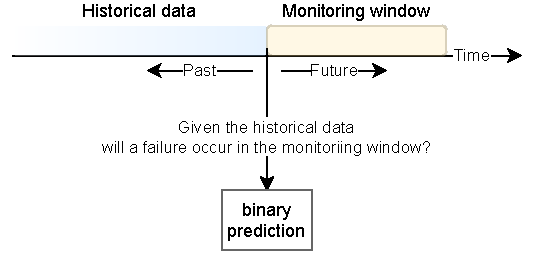
\includegraphics{approaches_failure_prediction_concept.pdf}
\caption{}
\end{subfigure}\\[1ex]
\begin{subfigure}{.5\linewidth}
\centering
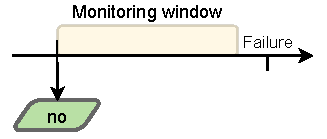
\includegraphics{approaches_failure_prediction_example_neg.pdf}
\caption{}
\end{subfigure}
\begin{subfigure}{.5\linewidth}
\centering
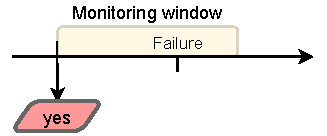
\includegraphics{approaches_failure_prediction_example_pos.pdf}
\caption{}
\end{subfigure}
\caption{Illustration of failure prediction:
        (a) general concept;
        (b) example of negative prediction, i.e. failure won't occur;
        (c) example of positive prediction, i.e. failure will occur.}
\label{fig:approaches_failure_prediction_illustration}
\end{figure}

Failure prediction is an approach where the goal is to make a binary prediction whether a failure will happen in near future --- in a monitoring window.
The concept of failure prediction is illustrated in the Figure 
\ref{fig:approaches_failure_prediction_illustration}.
Failure prediction approach is suitable in cases when there are available data about failures and when there are some patterns that precede the failure --- e.g. when an air compressor raises low pressure alarms before it fails.

\begin{figure}
    \includegraphics[width=.8\textwidth, keepaspectratio]{%
        approaches_failure_prediction_example_windows.pdf}
    \centering
    \caption{Illustration of monitoring, prediction and warning windows.}
    \label{fig:approaches_failure_prediction_example_windows}
\end{figure}

When predicting a failure, the domain problem might require the predictions to be made at least some time prior to the failure, e.g. the technicians have to be informed at least two days ahead in order to be able to schedule and perform the maintenance.
Therefore, a warning window might be specified which marks the minimal time prior to the failure in order for the prediction to be considered useful.
The time period of useful predictions is then called a prediction window and is defined as the time period between $t_F - M$ and $t_F - W$, where $t_F$ is a time stamp of the failure, $M$ is the size of the monitoring window and $W$ is the size of the warning window.
Figure \ref{fig:approaches_failure_prediction_example_windows} illustrates prediction and warning windows.

Failure prediction can be seen as a special case of fault detection where the prediction window are range-based faults.
However, failure prediction has some specifications in modeling and evaluation that differ from the range-based faults detection and thus we describe it as a special approach.

The concept of failure prediction is also used in many other domains such as healthcare, where heart failures are predicted, and it can also be found under name of early fault detection, early prediction of rare event, rare events prediction or rare events classification
\cite{ng2016early,weiss1998learning,ranjan2018dataset,choi2017using}.
In this thesis we will stick to the name failure prediction.

% TODO: add more literature that uses failure prediction and mention what other names they use for warning window etc.

\subsection{Data Specifications}

\begin{table}
	\centering
	\begin{tabular}{|c|c|cccc|c|}
    \hline
    subject id
    & time
    & \multicolumn{4}{|p{4cm}|}{\centering features}
    & failure event\\
    \hline
    subject 1 & 2020-01-01 &          0.1 &         0.05 & $\cdots$ &  34.1 & none \\
	subject 1 & 2020-01-02 &          0.3 &         0.12 & $\cdots$ &  34.2 & none \\
    $\vdots$ & $\vdots$ & $\vdots$ & $\vdots$ & $\ddots$ & $\vdots$ & $\vdots$ \\
    subject 1 & 2020-05-06 &          1.1 &         3.2 & $\cdots$ &  37.5 & none \\
    subject 1 & 2020-05-07 &          1.2 &         3.1 & $\cdots$ &  37.9 & failure A \\
    subject 1 & 2020-05-08 &          0.2 &         0.02 & $\cdots$ &  33.1 & none \\
    subject 1 & 2020-05-09 &          0.3 &         0.05 & $\cdots$ &  33.5 & none \\
    $\vdots$ & $\vdots$ & $\vdots$ & $\vdots$ & $\ddots$ & $\vdots$ & $\vdots$ \\
    subject 1 & 2020-07-29 &          2.5 &         0.21  & $\cdots$ &  35.9 & none \\
    subject 1 & 2020-07-30 &          2.2 &         0.2  & $\cdots$ &  36.1 & failure B \\
    $\vdots$ & $\vdots$ & $\vdots$ & $\vdots$ & $\ddots$ & $\vdots$ & $\vdots$ \\
	\end{tabular}
    \caption{A example of run-to-failure data set for failure prediction.}
    \label{tab:pdm_data_run_to_failure}
\end{table}

Data for training a failure prediction model must contain information about failures.
The data typically consist a condition monitoring data that are continuously collected during time and a failure log --- information when failures happened.
Such data are often called run-to-failure.
An example of run-to-failure data is illustrated in Table \ref{tab:pdm_data_run_to_failure}.
Moreover, it is necessary to have monitoring and warning windows.
However, it is good to note that the monitoring time does not have to be fixed.
Multiple models with different monitoring windows can be built and the choice of the final monitoring window can be made based on how the individual models perform.

\begin{figure}[H]
    \includegraphics[width=\textwidth, keepaspectratio]{%
        approaches_failure_prediction_modeling.pdf}
    \centering
    \caption{Diagram of modeling failure detection as time series
             point-based classification.}
    \label{fig:approaches_failure_prediction_modeling}
\end{figure}

\subsection{Modeling}

% \begin{figure}
%     \includegraphics[width=\textwidth, keepaspectratio]{%
%         approaches_failure_prediction_regression.png}
%     \centering
%     \caption{TODO}
%     \label{fig:approaches_failure_prediction_regression}
% \end{figure}

A failure prediction model can be built using a supervised classification algorithm where the samples in the training data are artificially labelled prior to the failure as positive.
Moreover, the predictions can be smoothed.
The whole modeling process is visualized in Figure
\ref{fig:approaches_failure_prediction_modeling} and described below.

\subsubsection{Artificial Labeling}

The classifier should learn to predict positive samples prior to failures.
Therefore, samples up to $M$ time steps prior to a failure are labeled as positive.
An example of artificial labeling with monitoring window of size 6 is illustrated in the upper part of Figure \ref{fig:approaches_failure_prediction_modeling}.

\subsubsection{Prediction}

The predictions are made point-wise by the trained classifier.
However, it might happen that there occur a single positive prediction among negative predictions due to a noise.
Therefore, the predictions can be smoothed using a rolling window and a positive prediction is assigned at time point $t$ when the ratio of positive predictions in the last $n$ predictions is higher  or equal than a given threshold.
We call the two parameters mentioned above a smoothing window and a smoothing threshold.
In case the classifier is capable of predicting probabilities of classes, the smoothing can be performed on the probabilities before the decision threshold is applied to avoid having two thresholds.

\subsection{Evaluation}
\label{sec:approaches_failure_prediction_evaluation}

In this section we describe how to evaluate the performance of a failure prediction model.
During evaluation we will aim to answer following questions:
\begin{itemize}
    \item What is the probability that the model will detect a failure?
    \item What is the probability that the model will make a false alarm? I.e. makes positive prediction but the failure won't occur in the monitoring window.
\end{itemize}
These questions are in \acrshort{ml} commonly answered by precision and recall metrics.
However, since we have more positive labels than failures due to artificial labeling, it is not straightforward how to use these metrics.
Below, we describe how to use classical precision and recall (described in Section \ref{sec:ml_evaluation}) and range-based precision and recall (described in Section \ref{sec:approaches_fault_detection_evaluation}) to evaluate a failure prediction model.
Next, we describe a modification of precision and recall, reduced precision and recall, introduced by Weiss et al. \cite{weiss1998learning}.
Finally, we propose new precision and recall metrics, a combination of the range-based metrics and the reduced metrics, that we call event-based precision and recall.

\subsubsection{Classical Precision and Recall}
\label{sec:approaches_failure_prediction_evaluation_classical_metrics}

This section describes how to use precision and recall using their standard definition (Section \ref{sec:ml_evaluation}) for failure prediction.

\begin{figure}
    \includegraphics[width=\textwidth, keepaspectratio]{%
        approaches_failure_prediction_evaluation.pdf}
    \centering
    \caption{Illustration of true labels and predictions in failure prediction.}
    \label{fig:approaches_failure_prediction_evaluation}
\end{figure}

As we use artificially created positive labels, we define following: 
\begin{enumerate}
    \item Actual positive samples are samples in the prediction windows, i.e. between $t_F - M$ and $t_F - W$.
    \item Actual negative samples are samples before $t_F - M$.
    \item Samples in the warning window, i.e. between $t_F - W$ and $t_F$, are not omitted from evaluation as they do not represent useful predictions.
\end{enumerate}

Figure \ref{fig:approaches_failure_prediction_evaluation} illustrates what time points are considered as positive and negative and which predictions are considered as \acrshort{tp}, \acrshort{tn}, \acrshort{fp} and \acrshort{fn}.
Recall and precision metrics are then used by their standard definition as:
\begin{align*}
    \text{recall} &= \frac{\text{TP}}{\text{P}},\\
    \text{precision} &= \frac{\text{TP}}{\text{TP} + \text{FP}}.
\end{align*}

\begin{figure}[hbt!]
    \includegraphics[width=.9\textwidth, keepaspectratio]{%
        approaches_failure_prediction_evaluation_recall_con.pdf}
    \centering
    \caption{Different predictions for the same data having the same recall score:
             (\textbf{left}) all of the three failures predicted
             (\textbf{right}) only one failure predicted.}
    \label{fig:approaches_failure_prediction_evaluation_recall_con}
\end{figure}

\begin{figure}[hbt!]
    \includegraphics[width=.75\textwidth, keepaspectratio]{%
        approaches_failure_prediction_evaluation_precision_con.pdf}
    \centering
    \caption{Different positions of two FPs having different severity:
             (\textbf{top}) far from each other
             --- such FPs can be considered as independent;
             (\textbf{middle}) close to each other
             --- the second FP is less serious and the two FPs can be almost
             considered as one;
             (\textbf{bottom}) close to each other and close to the monitoring period
             --- probably not so serious FPs as it might happen that the failure
             was predicted a bit sooner than at $t_F - M$.}
    \label{fig:approaches_failure_prediction_evaluation_precision_con}
\end{figure}

The classical metrics have two major issues:
\begin{itemize}
    \item Recall doesn't reflect how many failures were predicted.
    Figure \ref{fig:approaches_failure_prediction_evaluation_recall_con} shows examples of two models whose predictions have same recall score but they successfully predicted different number of failures.
    \item Precision doesn't reflect how close FPs are to each other.
    Figure \ref{fig:approaches_failure_prediction_evaluation_precision_con} shows examples of three series all having two \acrshort{fp}s but possibly having different importance in practice, e.g. two consecutive FPs may be treated as one FP whereas two FPs far from each other should count as two FPs.
\end{itemize}
Below, we describe three other types of precision and recall metrics that might mitigate these issues.

\subsubsection{Range-based Precision and Recall}

Failure prediction can be evaluated using range-based precision and recall as described in Section \ref{sec:approaches_fault_detection_evaluation} by taking the prediction windows as real fault (anomaly) ranges and consecutive positive predictions as predicted ranges.
Setting a non-zero existence weight $\alpha$ to the detection score of the range-based metrics solves the first issue mentioned above --- recall not reflecting how many failures were predicted.

\subsubsection{Reduced Precision and Recall}

Weiss et al. introduced in 1998 evaluation metrics called reduced precision and recall for prediction of rare events in time series \cite{weiss1998learning} which is a problem identical to failure prediction.
The main idea of the reduced metrics is to use the number of events (failures) instead of positive samples, use the number of predicted events instead of TP and use discounted FP instead of FP.

\paragraph{P $\rightarrow$ TotalEvents}
The total number of events (failures) is used instead of positive samples.
This means that for every prediction window consisting of $M - W$ samples there is one even, i.e. total number of events is equal to dividing the number of positives by the size of a prediction window.

\begin{figure}
    \centering
    \begin{subfigure}{.45\textwidth}
        \centering
        \includegraphics[width=.7\linewidth]{%
            approaches_failure_prediction_evaluation_failure_predicted.pdf}
        \caption{Failures predicted}
      \label{fig:approaches_failure_prediction_evaluation_failure_predicted}
    \end{subfigure}%
    \begin{subfigure}{.45\textwidth}
        \centering
        \includegraphics[width=.7\linewidth]{%
            approaches_failure_prediction_evaluation_failure_not_predicted.pdf}
        \caption{Failures not predicted}
        \label{fig:approaches_failure_prediction_evaluation_failure_not_predicted}
    \end{subfigure}
    \caption{Illustrations of events (failures) being and not being predicted}
\end{figure}

\paragraph{TP $\rightarrow$ EventsPredicted}
The true positives are replaced by the number of predicted events.
The event is considered as predicted when there is at least one positive prediction in its prediction window, i.e. at least $W$ and at most $M$ time steps prior to the event.
Figures \ref{fig:approaches_failure_prediction_evaluation_failure_predicted} and \ref{fig:approaches_failure_prediction_evaluation_failure_not_predicted} illustrate examples of events being predicted and not being predicted, respectively.

\begin{figure}
    \includegraphics[width=.75\textwidth, keepaspectratio]{%
        approaches_failure_prediction_evaluation_discounted_fp.pdf}
    \centering
    \caption{Illustration of calculating DiscountedFP.}
    \label{fig:approaches_failure_prediction_evaluation_discounted_fp}
\end{figure}

\paragraph{FP $\rightarrow$ DiscountedFP}
Every positive prediction has a meaning that an event (failure) will happen in the monitoring window.
If there are two consecutive positive predictions, the latter prediction can be considered as having lesser severity as the two consecutive predictions can be regarded as one false alarm.
Therefore, Weiss et al. define calculate as the number of complete, non-overlapping, monitoring windows associated with a false positive \cite{weiss1998learning}.
For example when having monitoring window of size 10, two consecutive false positives will produce a discounted FP of 1.1, i.e. 1 for the first prediction plus 0.1 for the second.
If the there is a false positive at time point $t$ and a false positive at time point $t + 5$, then the discounted FP for these two false positives will be equal 1.5.
Figure \ref{fig:approaches_failure_prediction_evaluation_discounted_fp} illustrates how discounted FP is calculated in three different scenarios.

The reduced precision and recall metrics are then defined as:
\begin{align*}
    \text{reduced recall} &= \frac{\text{EventsPredicted}}{\text{TotalEvents}},\\
    \text{reduced precision} &=
    \frac{\text{EventsPredicted}}
    {\text{EventsPredicted} + \text{DiscountedFP}}.
\end{align*}

Reduced recall is then identical to range-based precision when setting $\alpha = 1$, i.e. taking into account only the existence of a positive prediction in the prediction window.

\subsubsection{Event-based Precision and Recall}

Above, we described how range-based and reduced metrics can be used for failure prediction.
In this section, we propose a combination of the range-based and the reduced metrics.
The combination consists in taking the reduced metrics replacing the number of events predicted by a sum of detection scores from the range-based metrics.
We call such metrics event-based precision and recall and define it as follows:
\begin{align*}
    \text{event-based recall} &= \frac{\sum\text{DetectionScore}}{\text{Events}},\\
    \text{event-based precision} &=
    \frac{\sum\text{DetectionScore}}
    {\sum\text{DetectionScore} + \text{DiscountedFP}}.
\end{align*}
where $\sum\text{DetectionScore}$ is a sum of detection scores for all the prediction windows.
\section{Remaining Useful Life Prediction}
\label{sec:approaches_prognostics}

\Acrfull{rul} prediction is a \gls{pdm} approach where the goal is to predict the time left until the subject is still able to perform its intended function, i.e. until a failure occurs.
This section is structured as follows.
In Section \ref{sec:approaches_rul_motivation} we give a motivation why and when to predict \acrshort{rul} instead of using fault detection or failure prediction approaches.
In Section \ref{sec:approaches_rul_approaches} we describe and compare two different modeling approaches to \acrshort{rul} prediction --- \acrshort{hi}-based \acrshort{rul} prediction and direct \acrshort{rul} prediction.
The two approaches fundamentally differ in how \acrshort{rul} is predicted.
However, they still provide the same output --- the \acrshort{rul} of the subject --- and thus can be evaluated the same way.
Therefore, in the Section \ref{sec:approaches_rul_evaluation} we describe how to evaluate the \acrshort{rul} prediction independently on the chosen modeling approach.

\subsection{Motivation}
\label{sec:approaches_rul_motivation}

An accurate long term \acrshort{rul} prediction can significantly help in scheduling the maintenance actions in comparison with fault detection or failure prediction approaches.
Imagine a situation of having a large amount of subjects which started operating at the same time --- for example a fleet of one hundred wind turbines.
If the turbines were operating under similar conditions it might happen that they will all tend to fail after similar amount of time of operation --- e.g. after two years.
Both fault detection and failure prediction approaches would then notify that all the wind turbines are faulty (or are going to fail soon) at a similar time shortly before the failures, let's say one week ahead.
However it might be impossible to schedule maintenance actions for all the wind turbines at that time point because only two wind turbines can be maintained per day and there is one hundred of wind turbines about to fail in one week.
With an accurate \acrshort{rul} prediction, on the other hand, one can continuously have information about when each individual subject is going to fail.
If the \acrshort{rul} is then similar for many subjects the maintenance actions can be scheduled more in advance so that all the subjects are maintained in advance.
However, an accurate \acrshort{rul} prediction is typically possible only in certain domains and only when having the right type of data.

\Acrshort{rul} prediction is typically done on subjects which have an ongoing continuous degradation that can be well quantified --- for example a turbine bearing deterioration.
The failure then can be either a complete inability of the subject to operate (e.g. the wind turbine shuts down) or it can be a state when the subject is no longer capable of safe operation or of operation at enough quality --- e.g. a maximum capacity of a battery reaches 40 \% of the designed capacity\footnote{In such cases the failure is often rather called an end of life (EoL). However, as it principally represents the same thing we will stick to the naming convention of failure.}.
In such cases it is common to predict \acrshort{rul} during the whole lifetime of the subject (e.g. every day or week) \cite{miao2013remaining}.
In other cases, however, the subject might operate under stable, healthy, conditions without any sings of wear until a fault occurs which triggers the degradation process --- the fault grows in severity (as illustrated in the beginning of this chapter in Figure \ref{fig:approaches_intro_health_stages}).
In such cases the \acrshort{rul} can be predicted over the whole lifetime as well but it might happen that the prediction would be highly inaccurate until the fault occurs.
Therefore, the \acrshort{rul} prediction can 
start after the fault (or anomaly) is detected\footnote{assuming the fault is detected early enough so that the \acrshort{rul} prediction is useful} \cite{lei2018machinery} and thus providing an estimation of the fault's severity.

\subsection{Approaches}
\label{sec:approaches_rul_approaches}

We identified two different modeling approaches to \acrshort{rul} prediction --- direct RUL prediction and HI-based RUL prediction\footnote{HI --- health indicator}.
In this section we describe and compare the two approaches.

% Before we proceed to their description, however, we want to shortly comment on the naming of the approaches.
% There is very few literature that mentions the existence of the both approaches.
% Typically only one of the approaches is used (or described) and it is simply referred to both of them as \acrshort{rul} prediction \cite{miao2013remaining, hu2012ensemble, klausen2018novel,  yang2016health}.
% The first approach, the \acrshort{hi}-based \acrshort{rul} prediction, can be considered as a classical approach to \acrshort{rul} prediction as there is much more literature using this approach and 

% The first approach consists in construction of a \acrfull{hi} from the condition monitoring data, forecasting its future values and predicting when the \acrshort{hi} crosses a predefined failure threshold.
% In this approach it is common that a separate model is build for every subject and the model is updated with each new health indicator value \cite{lei2018machinery}.
% The second approach consists in direct prediction of the \acrshort{rul} from the condition monitoring data using a regression model.
% The regression model is trained on historical run-to-failure data of subjects from which their \acrshort{rul} is calculated.
% Unfortunately, 
% % The first approach, utilizing the \acrshort{hi}, is sometimes referred to as prognostics  \cite{lei2018machinery, lee2014prognostics} but the definition of prognostics is that it is a \acrshort{rul} prediction \cite{lei2018machinery}.
% % The second approach is sometimes referred to as regression approach to \acrshort{rul} prediction \cite{babu2016deep} but as will be described later in this section even the first approach can utilize regression models.
% The only work we found that tries to distinguish between the approaches \cite{jia2018review} calls them "Unsupervised Prognosis" and "Supervised RUL Prediction".
% However, that is highly ambiguous naming as first approach can utilize supervised learning algorithms as well and as the prognosis and \acrshort{rul} prediction are equivalent.
% Therefore, we decide to call the two approaches an \acrshort{hi}-based \acrshort{rul} prediction and a direct \acrshort{rul} prediction.
% We describe and compare both of the approaches in more detail in Section  \ref{sec:approaches_rul_approaches}.

\subsubsection{Direct \acrshort{rul} Prediction}
\label{sec:approaches_rul_direct}

\begin{table}
	\centering
	\begin{tabular}{|c|c|ccc|c|c|c|}
    \hline
    subject id
    & time
    & \multicolumn{3}{|p{3cm}|}{\centering features}
    & failure
    & \textbf{RUL}\\
    \hline
    subject A & 2020-01-01 &          0.1 & $\cdots$ &  34.1 & 0 & 127\\
	subject A & 2020-01-02 &          0.3 & $\cdots$ &  34.2 & 0 & 126\\
    $\vdots$ & $\vdots$ & $\vdots$ & $\ddots$ & $\vdots$ & $\vdots$ & $\vdots$\\
    subject A & 2020-05-05 &          1.1 & $\cdots$ &  37.5 & 0 & 2\\
    subject A & 2020-05-06 &          1.1 & $\cdots$ &  37.5 & 0 & 1\\
    subject A & 2020-05-07 &          1.2 & $\cdots$ &  37.9 & 1 & 0\\
    \hdashline
    subject B & 2020-01-01 &          0.2 & $\cdots$ &  33.1 & 0 & 89\\
    subject B & 2020-01-02 &          0.3 & $\cdots$ &  33.5 & 0 & 88\\
    $\vdots$ & $\vdots$ & $\vdots$ & $\ddots$ & $\vdots$ & $\vdots$ & $\vdots$\\
    subject B & 2020-03-29 &          2.5 & $\cdots$ &  35.9 & 0 & 1\\
    subject B & 2020-03-30 &          2.2 & $\cdots$ &  36.1 & 1 & 0\\
    \hline
	\end{tabular}
    \caption{Example of calculating the \acrshort{rul} values from the run-to-failure data.}
    \label{tab:pdm_data_run_to_failure}
\end{table}

Direct \acrshort{rul} prediction is suitable when there are available run-to-failure data for at least several subjects.
The approach consists in training a regression model on the run-to-failure data where the regressands (features) can be any known data about the subject at the time of the prediction and the regressor (the predicted value) is the \acrshort{rul} retrospectively calculated from the run-to-failure data.
The calculation of the RUL is typically done as follows --- at the time of the failure, $T$, the RUL is equal to 0, at time $T-1$ the RUL is equal to 1, at $T-2$ the RUL is equal to 2 and so on.
Table \ref{tab:pdm_data_run_to_failure} shows an example of run-to-failure data set and calculating of the RUL.

As described in the previous section, the subjects might operate under stable and healthy conditions until a fault occurs which triggers the degradation process.
In that case the RUL prediction might be very inaccurate at the early stage of the subject's operation where it might be hard to distinguish between e.g. RUL of 200 days and 170 days.
Therefore in some works limiting of the \acrshort{rul} values with an upper bound is suggested \cite{jayasinghe2018temporal} --- e.g. all the RUL values above 130 are set to 130  see Figure \ref{fig:approaches_rul_clipping} for illustration).
The authors in \cite{jayasinghe2018temporal} conclude that such clipping might result in better performance in terms of root mean squared error metric.
However, as will be discussed in Section \ref{sec:approaches_rul_evaluation} the RMSE metric might be unsuitable for evaluation of RUL prediction performance and thus it is questionable whether this RUL clipping helps the overall performance of the model.

\begin{figure}
    \centering
    \includegraphics[width=.6\textwidth, keepaspectratio]{%
        approaches_rul_clipping.png}
    \caption{Illustration of limiting RUL with an upper bound \cite{jayasinghe2018temporal}.}
    \label{fig:approaches_rul_clipping}
\end{figure}

\begin{figure}
    \centering
    \includegraphics[width=.6\textwidth, keepaspectratio]{%
        approaches_rul_bayesian.png}
    \caption{Illustration of RUL prediction with a Bayesian LSTM neural network  \cite{louw2018remaining}.}
    \label{fig:approaches_rul_bayesian}
\end{figure}

Promising results of direct RUL prediction have been achieved with recurrent and convolutional neural networks in various domains such as wind turbines or bearings \cite{mahamad2010predicting, babu2016deep}.
In recent years, Bayesian neural networks are gaining on interest in direct RUL prediction as they can predict a \gls{pdf} instead of single value predictions \cite{peng2019bayesian, louw2018remaining}.
The mean of the \gls{pdf} can then be used as the predicted RUL and a confidence interval can be calculated and used as a form of uncertainty --- which might be very valuable for the end users as a supportive information about the prediction.
Figure \ref{fig:approaches_rul_bayesian} illustrates prediction of \gls{rul} with a Bayesian LSTM neural network.

In some literature, the direct \acrshort{rul} prediction approach is considered as having relatively low capability of predicting the \acrshort{rul} since a linear relationship between the \acrshort{rul} and the condition monitoring data is established \cite{jia2018review}.
% However, we must emphasize that the linear relationship holds only when using raw data and a linear model.
% When a more complex model such as SVM with higher degree polynomial kernel or an artificial neural network is used or when some feature engineering is performed (e.g. squared age of the subject is used as a feature), the mentioned linear relationship no longer holds.

\subsubsection{\acrshort{hi}-based \acrshort{rul} Prediction}
\label{sec:approaches_rul_hi_based}

The \acrshort{hi}-based \acrshort{rul} prediction approach is suitable in cases when there is available a \acrfull{hi} that directly represents the subject's health state and a predefined failure threshold.
The failure of the subject is then considered as the time point when the \acrshort{hi} crosses the failure threshold.
A typical example of such case are batteries where the health indicator can be their current maximal capacity and the failure threshold can be a ratio of the designed maximal capacity (e.g. 30 \%).
% Another example are bearings where the health indicator can be root mean square of vibration data and the failure threshold can be some maximal permissible vibration level --- e.g. ISO norm \cite{iso_mechanical} even defines permissible thresholds for some bearings.
The \acrshort{rul} prediction then consists in building a model that forecasts future values of the \acrshort{hi} and in identifying the time point when the HI crosses the failure threshold.
The RUL is then calculated as the time difference between the identified time point of the crossing and the current time point.

\begin{figure}
    \centering
    \includegraphics[width=\textwidth, keepaspectratio]{%
        approaches_rul_prognostics_example.png}
    \caption{Illustration of \acrshort{hi}-based \acrshort{rul} prediction.
             The red dashed line represents a failure threshold (FT), the blue line
             represents a health indicator up to a current time point (green dot), the green
             line shows a prediction of the health indicator in the future and
             the red line represents the actual future values of the health indicator.
             \cite{lei2018machinery}.}
    \label{fig:approaches_rul_prognostics_example}
\end{figure}

The forecasted \acrshort{hi} is commonly in a form of a \acrfull{pdf} which tends to have higher variance the farther to the future the \acrshort{hi} is predicted \cite{saxena2010metrics}.
In case of predicting the \gls{pdf} of the HI the failure can be defined as the time point when the mean of the \acrshort{pdf} crosses the failure threshold.
Figure \ref{fig:approaches_rul_prognostics_example} illustrates the forecasting of the \acrshort{hi} with a \acrshort{pdf}.

The HI forecasting techniques can be divided into two categories:
\begin{itemize}
    \item model-based techniques;
    \item machine learning techniques;
\end{itemize}

\begin{figure}
    \centering
    \includegraphics[width=.7\textwidth, keepaspectratio]{%
        intro_pdm_battery_degradation.jpg}
    \caption{Finding an empirical model for degradation of battery capacity 
             \cite{miao2013remaining}.}
    \label{fig:approaches_rul_battery}
\end{figure}

\paragraph{Model-based Techniques}
The model-based techniques are based on the existence of an underlying physical or statistical model that describes the degradation process of the subject.
Such physical or statistical models can be either apriori known or empirically observed from the available data.
For example the capacity of the batteries can be commonly fitted by an exponential model \cite{he2011prognostics} --- see Figure \ref{fig:approaches_rul_battery} for illustration.
The physical and statistical models have typically parameters which are estimated from the currently available HI data of the subject (the parameters are estimated for each subject separately).
In other words the forecasting at time point $t$ is done by a model with parameters estimated based on the HI data up to time point $t$.

\paragraph{ML Techniques}
The AI techniques, on the other hand, do not require any domain knowledge about the degradation process but rather build a model that learns the degradation patterns from the previous HI data points by itself.
A simple technique can be using a regression model that takes time as the regressand and the HI as the regressor \cite{yoo2018novel}.
More advanced techniques include for example a recurrent neural networks which can be trained to time series prediction, i.e. output future values of the HI based on previous values \cite{zhang2018long}.

% TODO: Uber extreme forecasting

A big benefit of HI-based RUL prediction over the direct RUL prediction is that there is no need for run-to-failure data.
The unavailability of run-to-failure data is common in many domains such as aviation where the subjects simply cannot operate until a failure mostly from safety reasons \cite{saxena2010metrics}.
On the other hand, the downside of the HI-based RUL prediction is that there has to be a well defined health indicator and failure threshold.

\subsection{Evaluation}
\label{sec:approaches_rul_evaluation}

In this section, we describe how to evaluate the performance of a RUL prediction model.
We will use the following notation:
\begin{itemize}
    \item $N$ --- number of subjects;
    \item $n \in [1, N]$ --- index of a n-th subject;
    \item $t \in [1, T_n]$ --- time index of n-th subject's observations, where $t=1$ is the first observation and $t=T_n$ is the time stamp of the failure;
    \item $\text{RUL}_n(t)$ --- actual \gls{rul} of n-th subject at time $t$;
    \item $\widehat{\text{RUL}}_n(t)$ --- predicted \gls{rul} of n-th subject at time $t$;
    \item $W$ --- warning time;
    \item $\text{EoUP}_n = T_n-W$ --- \acrfull{eoup}, the last time stamp of useful predictions, i.e. not yet in the warning window.
\end{itemize}
The warning time has the same meaning as in failure prediction --- some lead time before the failure of the subject might be necessary so that the maintenance action can be scheduled and performed.
Therefore, we will exclude the time points between $T-W$ and $T$ from the evaluation.

% The performance of \acrshort{rul} prediction can be evaluated on four levels:
% \begin{enumerate}
    
%     \item single prediction level --- what is the error of the prediction from the actual RUL?
    
%     \item \acrshort{rul} level --- what is a typical error of predicting a specific actual \acrshort{rul} value? (e.g. how accurate are the predictions when actual RUL value is 100 days vs 10 days);
%     % \item relative \acrshort{rul} level --- what is a typical error of the model when
%     %       predicting a specific actual \acrshort{rul} value (e.g. a mean error
%     %       of predictions for the actual \acrshort{rul} of 100 days is 10 days);
    
%     \item subject level --- how accurate is the model in predicting \acrshort{rul} of a specific subject?;
    
%     \item data set level --- what is the overall performance of the predictions on the whole data set, e.g. on a fleet of subjects?;

% \end{enumerate}
% Below we will describe various evaluation metrics and techniques and we will describe how they can be used for evaluation at the different levels mentioned above.

% The \acrshort{rul} predictions are made for every subject while the predicted values 
% Each prediction is made for a specific time stamp of a specific subject.

\subsubsection{Classical Metrics}

\Acrshort{rul} prediction is in context of \acrshort{ml} a regression task --- the goal is to predict a continuous variable.
Thus, classical regression metrics such as MAE, RMSE or MAPE can be used.
However, it is not straightforward how to use them from two reasons.
First, we should omit the predictions made in the warning window, the predictions after \acrshort{eoup}.
Second, we can calculate the mean error either over subjects or over individual samples.

An absolute error, squared error and absolute percentage error for n-th subject can be calculated as:
\begin{align*}
    \text{AbsoluteError}_n &= \sum_{t=1}^{\text{EoUP}_n}\left|\text{RUL}_n(t) - \widehat{\text{RUL}}_n(t)\right|,\\
    \text{SquaredError}_n &= \sum_{t=1}^{\text{EoUP}_n}{(\text{RUL}_n(t) - \widehat{\text{RUL}}_n(t))^2},\\
    \text{AbsolutePercentageError}_n &= \sum_{t=1}^{\text{EoUP}_n}\left|\frac{\text{RUL}_n(t) - \widehat{\text{RUL}}_n(t)}{\text{RUL}_n(t)}\right|.\\
\end{align*}
In general, we will denote the error of the n-th subject as Error$_n$.
The mean of the errors can be then calculated either over subjects or over samples:
\begin{align*}
    \text{mean error over subjects} &= \frac{1}{N}\sum_{n=1}^{N}\frac{\text{Error}_n}{\text{EoUP}_n},\\
    \text{mean error over samples} &= \frac{1}{\sum_{n=1}^N{{\text{EoUP}_n}}}\sum_{n=1}^{N}{\text{Error}_n}.\\
\end{align*}

Mean absolute percentage error (MAPE) over samples can be then calculated as:
\begin{align*}
    \text{MAPE} = \frac{1}{\sum_{n=1}^N{{\text{EoUP}_n}}}\sum_{n=1}^{N}{\sum_{t=1}^{\text{EoUP}_n}\left|\frac{\text{RUL}_n(t) - \widehat{\text{RUL}}_n(t)}{\text{RUL}_n(t)}\right|}
\end{align*}
The metrics such as MAE and RMSE are then calculated analogically.

% Typically, the lower the actual \acrshort{rul} is the more accurate the predictions should be --- e.g. it is much less severe error if the actual \acrshort{rul} is 200 days and the prediction is 220 days in comparison with an actual \acrshort{rul} being 5 days and the prediction being 25 days.
% This exactly reflects MAPE metric which scales the errors accordingly to the actual predicted value.

\subsubsection{Prognostic Horizon}

\begin{figure}
    \centering
    \includegraphics[width=\textwidth, keepaspectratio]{%
        approaches_rul_evaluation_prognostic_horizon.pdf}
    \caption{Illustration of prognostic horizon.}
    \label{fig:approaches_rul_evaluation_prognostic_horizon}
\end{figure}

Prognostic horizon is an evaluation metric specifically tailored for \acrshort{rul} prediction proposed by Saxena et al. \cite{saxena2010metrics}.
It aims to answer the following question: What time ahead of the failure are the predictions within a prespecified bound around the actual \acrshort{rul} for one specific subject?
The prognostic horizon is defined as the time difference between the time of failure ($T_n$) and the first time index from which all the future predictions are within the boundaries specified by parameter $\alpha$.
For the n-th subject the prognostic horizon (PH) with parameter $\alpha$ is defined as:
\begin{align*}
    \text{PH}_{\alpha, n} &= T - \min\left\{i|
        \forall t, t \geq i : \widehat{\text{RUL}}_n(t) \in [\text{RUL}_n(t) - \alpha, \text{RUL}_n(t) + \alpha]
  \right\}.
\end{align*}
Figure \ref{fig:approaches_rul_evaluation_prognostic_horizon} illustrates the calculation of prognostic horizon on predictions for one subject.

For evaluation of multiple subjects, \acrfull{mph}$_\alpha$ can be used as:
\begin{align*}
    \text{MPH}_\alpha = \frac{1}{N}\sum_{n}{\text{PH}_{\alpha, n}}
\end{align*}

\subsubsection{Metrics Relative to RUL}

% All the above mentioned metrics produce a single score.
% Therefore, when we obtain e.g. a score RMSE equal to 20, we do not know whether there were high errors at the beginning a

It might happen that the RUL prediction model has relatively high errors at high RUL values compared to the errors at low RUL values.
Therefore, we can calculate the errors only for RUL values lower than a certain fixed value, for example calculate MAPE only for RUL values lesser than 40.
We define a mean absolute percentage error up to RUL values equal to $k$ (MAPE@k) as:
\begin{align*}
    \text{MAPE@k} = \frac{1}{\sum_{n=1}^N{{\left(\text{EoUP}_n - k - 1 \right)}}}\sum_{n=1}^{N}{\sum_{t=k}^{\text{EoUP}_n}\left|\frac{\text{RUL}_n(t) - \widehat{\text{RUL}}_n(t)}{\text{RUL}_n(t)}\right|}
\end{align*}
Metrics such as MAE@k, RMSE@k can be then defined analogically.

In RUL prediction, we might be interested in how the model performs at relatively to the actual RUL values, i.e. we might want to obtain one score for every actual RUL value.
Therefore, instead of calculating a mean score over all the samples, we can calculate a mean score over all subjects at a various RUL values.
MAPE at different RUL values is defined as follows:
\begin{align*}
    \text{MAPE(RUL)} = \sum_n \frac{\text{RUL} - \widehat{\text{RUL}}_n(T_n - \text{RUL})}{\text{RUL}}.
\end{align*}
The metrics MAE, RMSE and others can be then defined analogically.

% TODO
% TODO

% Saxena et al. proposed a metric called relative accuracy \cite{saxena2010metrics} which measures the accuracy of the \acrshort{rul} prediction at a relative \acrshort{rul} value:
% \begin{align*}
%     \text{RelativeAccuracy}_\lambda = 1 - \frac{|y_{\lambda T} - \hat{y}_t|}{y_t}
% \end{align*}
% where $t_\lambda = \lambda T, \lambda \in [0, 1]$

% \begin{figure}
%     \centering
%     \includegraphics[width=\textwidth, keepaspectratio]{%
%         approaches_prognostics_relative_accuracy.pdf}
%     \caption{Relative accuracy}
%     \label{fig:approaches_prognostics_relative_accuracy}
% \end{figure}


\begin{figure}[H]
    \centering
    \includegraphics[width=\textwidth, keepaspectratio]{%
        approaches_rul_prediction_optimistic.pdf}
    \caption{Illustration of optimistic and pessimistic predictions.}
    \label{fig:approaches_rul_prediction_optimistic}
\end{figure}

\begin{figure}[H]
    \centering
    \includegraphics[width=.8\textwidth, keepaspectratio]{%
        approaches_rul_asymmetric_scoring.png}
    \caption{Asymmetric weighting function for late and early predictions \cite{saxena2008damage}.}
    \label{fig:approaches_rul_asymmetric_scoring}
\end{figure}

\subsubsection{Asymmetric Weighting}

When the prediction is not perfect, i.e. $\text{RUL} \neq \widehat{\text{RUL}}$, it can be either late (optimistic) if $\text{RUL} > \widehat{\text{RUL}}$ or early (pessimistic) if $\text{RUL} < \widehat{\text{RUL}}$.
Figure \ref{fig:approaches_rul_prediction_optimistic} illustrates RUL predictions for one subject and highlights what predictions are late and which are early.
The late predictions might bring a risk that the subject fails before the maintenance is performed.
Therefore, the early predictions are typically better since the subject is in the worst case maintained earlier than it would have to be.

In \cite{nectoux2012pronostia} and \cite{saxena2008damage} the authors suggest using an asymmetric weighting function for weighting the prediction errors.
The main idea is to give higher weight to the late predictions in comparison with the early ones.
The asymmetric weighting function $\varphi$ can be for example defined as
\begin{align*}
    \varphi(d) &= \begin{cases}
            -d &\text{ if } d < 0\\
            2d &\text{ if } d \geq 0
    \end{cases}
\end{align*}
where $d$ is the difference between the predicted RUL and actual RUL, i.e. $d = \widehat{\text{RUL}} - \text{RUL}$.
Figure \ref{fig:approaches_rul_asymmetric_scoring} illustrates the above defined asymmetric weighting function.

The weighting function $\varphi$ can be then used in the classical regression metrics.
We define a mean asymmetrically weighted percentage error (MAWPE) with an asymmetric scoring function $\varphi$ as:
\begin{align*}
    \text{MAWPE}_\varphi &= \frac{1}{\sum_{n=1}^N{{\text{EoUP}_n}}}\sum_{n=1}^{N}{\sum_{t=1}^{\text{EoUP}_n}\left|\varphi\left(\frac{\text{RUL}_n(t) - \widehat{\text{RUL}}_n(t)}{\text{RUL}_n(t)}\right)\right|} \\
\end{align*}
The usage of the asymmetric weighting function in other metrics is then analogical.

The asymmetry can be also applied in prognostic horizon where instead of a single parameter $\alpha$ (defining the width of the bound) two parameters $\alpha^+$ and $\alpha^-$ can be used which define the lower and the upper boundary, respectively.
\input{chapters/approaches/summary}
